% !TEX root = ../notes_template.tex
\chapter{Individual Movement} \label{sec:Chap4_movement}

\section{Movement Ecology} \label{sec:Chap4_movement_ecology}

All organisms must move at some point in their life. Examples include an Arctic tern (\textit{Sterna paradisaea}) migrating 40,000 km between the poles every year, an apple falling off the tree and rolling a meter before taking root, or freshwater mussel larvae that parasitize fish gills to hitch a ride upriver.  Given that movement is ubiquitous, the movement of organisms is important in (nearly) all ecological theories and is analyzed using a wide range of techniques.  For example:
\begin{itemize}
    \item The Island Theory of Biogeography derives area-diversity relationships from postulating some ongoing process by which species are transported from a mainland habitat (species pool) to an island \cite{macarthur_theory_1967};
 
    \item Optimal Foraging Theory seeks to identify those behaviors (e.g., foraging location and time spent feeding) that are expected to maximize individual fitness \cite{krebs_optimal_1978}, and from there predict how behaviors would change under alternative forage densities and predatory controls;
 
    \item Modern Coexistence Theory seeks to classify the mechanisms by which a population might persist over time, defining the correlation between productivity and density arising from a combination of habitat differences and dispersal abilities \cite{chesson_mechanisms_2000};

    \item The Movement Ecology Paradigm \cite{nathan_movement_2008} seeks to unify the analysis of movement for any organism by describing the organism's internal state, locomotive, sensory, cognitive, and navigational capabilities, and the external factors affecting movement.  
\end{itemize}
Clearly, any investigation of spatio-temporal processes in ecology must include some general approaches to study the movement of organisms that includes these various mechanisms.

Despite the ubiquity of movement in ecological theory, some theories and analytical methods include movement \textit{implicitly} while others do so \textit{explicitly}.  For example, models for population growth are often derived from implicit assumptions about how individuals are distributed spatially and how increases in local density inhibit population growth rates \cite{roughgarden_production_1997}.  By contrast, other ecological models explicitly represent the drivers and rates of individual movement, e.g., when representing population rescue in a meta-population model of checkerspot butterflies occurring in multiple habitat patches \cite{hanski_ecological_2017}.  Explicit movement models often proceed by tracking the movement of individuals between habitat patches or across continuous space, while implicit models often derive some steady-state properties of aggregate dynamics from proposed movement rules \cite{levin_theories_1997}.  Both approaches are useful, but aggregate (``implicit") properties can generally be obtained from an explicit movement model, while it is harder to go the other way (i.e., to identify an explicit movement process from a resulting spatial pattern).  We therefore focus the following on how to estimate movement explicitly, so that readers can then use estimates to simulate animal movement to generate aggregate (implicit) patterns.  In some cases, the aggregate patterns resulting from explicit movement assumptions can then be compared with population-scale data to refute or support hypothesized movement models.  

In Chapter \ref{Chap1}, we introduced Individual-Based Models (IBM) by demonstrating how population dynamics arise from birth and death timing of individuals, or habitat utilization arises from the location and size of individuals.  We similarly claimed that IBMs can be efficiently fitted to data by converting from this Lagrangian viewpoint (tracking changes in attributes for individuals over time) to an Eulerian viewpoint (tracking densities of animals based on their attributes). However, a full description of individual dynamics must also include how individual location changes over time.  Most ecological movements can be accounted for with three basic processes, each with its own simple mathematical expression:
\begin{enumerate}
    \item \textit{Taxis}\index{taxis}, where animals move intentionally and predictably toward their preferred habitats, and where the emphasis is upon identifying the habitat preference function that governs taxis;

    \item \textit{{Drift}}\index{drift}, where animals move along a known path, typically drifting due to their physical environment.  Passive drift occurs, e.g., for dispersal of pollen due to prevailing winds, or dispersal of aquatic larvae due to oceanographic currents.  Drift is also a generic term for directional movement where the habitat preference is not known or explicitly represented;
 
    \item \textit{Diffusion}\index{diffusion}, where animals move in a way that is not otherwise explained as taxis or passive drift, and therefore appears to be "random" relative to known or hypothesized movement drivers.  In the following, we use the term ``diffusion" both in its strict sense (i.e., using the Eulerian viewpoint, where densities tend to revert to the average of nearby locations) and a looser sense (i.e., using the Lagrangian viewpoint to represent diffusive movement for an individual following a random-walk process).
\end{enumerate}
Both taxis and drift are sometimes classified as \myindex{advection}.  However, we distinguish between these two components of advection for technical reasons that we will discuss later.  Similarly, diffusion is a statistical residual that remains unexplained after predicting movement based on advection.  It is therefore useful to start with a model of diffusion, and subsequently describe how we can attribute movement using other mechanisms.  For some ecological purposes, we might seek to describe taxis and drift so accurately that there is no remaining movement to describe as diffusion.  For other ecological analyses, however, it might not be necessary to account for taxis and drift explicitly, and we might be content by estimating a diffusion rate with no other mechanism involved. 

\section{Defining Diffusion and Taxis} \label{sec:Chap4_diffusion_and_taxis}

We start by defining location \(S_t\) along one dimension, \(S \in \mathbb{R}\) for an individual at any time \(t\)\footnote{See https://github.com/james-thorson/Spatio-temporal-models-for-ecologists/Chap\_4 for code associated with this chapter.}. We start by explaining all movement as ``diffusion", i.e., as a random-walk process that results in diffusive movement:

\begin{equation} \label{eq:Chap4_1d_difference_equation}
    S(t+\Delta_t) = S(t) + \delta    
\end{equation}
where:
\begin{equation} \label{eq:Chap4_delta}
    \delta \sim \mathrm{Normal}(0, \Delta_t \sigma^2)    
\end{equation}
and where \(\sigma^2\) is the rate of random movement such that the variance in displacement over interval interval \(\Delta_t\) is \(\Delta_t \sigma^2\).  We can instead write this using a diffusion coefficient \(D = \frac{\sigma^2}{2}\), although the random movement rate \(\sigma^2\) likely provides more intuition regarding the process involved.   

If we allow the length of time-intervals to approach zero (i.e., define movement in continuous time), then Eq. \ref{eq:Chap4_delta} defines a \myindex{Weiner process} such that \( \delta \sim \sigma W(\Delta_t) \).  We can use this to define a stochastic partial differential equation that generalizes Eq. \ref{eq:Chap4_1d_difference_equation} in continuous time:
\begin{equation} \label{eq:Chap4_brownian_motion}
    \partial S =  \sigma \partial W \partial t   
\end{equation}
such that \( \int_{0}^{\Delta_t} \sigma \partial W  \partial t = \delta \) where this \(\delta\) is the same as the one in Eq. \ref{eq:Chap4_1d_difference_equation}, and Eq. \ref{eq:Chap4_brownian_motion} is sometimes called \myindex{Brownian motion}.  The diffusion coefficient can then be related to the \textit{mean free path} of a hypothetical particle, i.e., how far a particle (e.g., an individual animal) typically goes before randomly determining a new direction of travel.    

In two or more dimensions, we then generalize this by defining location as vector \( \mathbf{s}_t \), and this location evolves as:

\begin{equation} \label{eq:Chap4_diffusion}
\begin{gathered}
    \mathbf{s}(t+\Delta_t) = \mathbf{s}(t) + \mathbf{\delta}    \\
    \mathbf{\delta} \sim \mathrm{MVN}( \mathbf{0}, \Delta_t \sigma^2 \mathbf{I})    
\end{gathered}
\end{equation}
where \(\Delta_t \sigma^2\) is the expected variance for each individual coordinate, and we could again write this using diffusion coefficient \(D=\frac{\sigma^2}{2}\).  We are defining \(\sigma^2\) as the variance rate for each individual dimension, so the mean-squared displacement (MSD) is the sum of squares across \(n\) spatial coordinates, such that:

\begin{equation} \label{eq:Chap4_MSD}
    MSD = \E( |\mathbf{s}(t+\Delta_t) - \mathbf{s}(t)| ) = 2nD \Delta_t
\end{equation}
where \(n\) is the number of dimensions.  This mean-squared displacement can then be compared with empirical data to infer mechanisms of animal dispersal \cite{skellam_random_1951,okubo_examples_2001}.

We next introduce taxis by defining a \myindex{habitat preference function} \( h(s) \).  This preference function is an imaginary property of each location, and can be defined based on local habitat, animal sensory capabilities, and other properties that are understood to affect animal movement \cite{nathan_movement_2008}. It is analogous to potential functions that are widely used in physics, e.g., a gravitational potential that accelerates bodies with mass or an electric potential that accelerates bodies with electric charge \cite{brillinger_learning_2012}.  For this reason, this preference function for describing taxis has been called a \textit{potential function} \cite{mcclintock_integrated_2022,preisler_modeling_2004}, although we prefer to use ecological vocabulary to describe the same process.  Animals seek to move toward locations with higher preference, so they tend to move up a gradient of the habitat preference function.  In the case of a single spatial dimension, we calculate this using the first derivative \(h'(S) = \frac{\mathrm{d}}{\mathrm{d} S}h(S) \) of the preference function \(h(S)\) at a given location \(S\):

\begin{equation} \label{eq:Chap4_1D_taxis}
  \partial S = h'(S) \partial t + \sigma W \partial t    
\end{equation}
However, we can write this more generally using a \myindex{gradient operator} \( \nabla h(S)\), which describes taxis in any number of spatial coordinates:

\begin{equation} \label{eq:Chap4_differential_equation}
    \partial \mathbf{s} = \nabla h(\mathbf{s}) \partial t + \sigma W \partial t    
\end{equation}
where \( \nabla h(\mathbf{s})\) replaces the derivative in Eq. \ref{eq:Chap4_1D_taxis}. For example, when defining movement in two dimensions such that location \( \mathbf{s}=(x,y) \), we can write this gradient as \( \nabla h(\mathbf{s}) = ( \frac{\partial}{\partial x} h(x,y), \frac{\partial}{\partial y} h(x,y) ) \).  Gradient \( \nabla h(\mathbf{s}) \) then returns a vector pointing in the direction of greatest increase in preference \(h(\mathbf{s})\), with vector length proportional to this gradient.  Given this definition, taxis represents the tendency for animals to move up the gradient of this habitat-preference function.  

In general, this SPDE can be solved exactly when preference \(h\) takes particular forms.  As outlined in Section \ref{sec:Chap1_IBMs}, however, we seek methods that we can apply regardless of the specific preference function being used.  To do so, we introduce the \myindex{Euler method} to discretize the path that arises from this process, which results in a \myindex{directed random walk}.  This involves replacing the differential equation (which must be solved via integration) with a difference equation (which can be solved via summation).  In this case, taxis during the interval \(\Delta_t\) is based only on habitat preference at the the begin of the interval:

\begin{equation} \label{eq:Chap4_difference_equation}
    \mathbf{s}(t+\Delta_t) - \mathbf{s}(t) =  \nabla h(\mathbf{s}(t)) \Delta_t + \delta    
\end{equation}
Eq. \ref{eq:Chap4_difference_equation} is conceptually identical to Eq. \ref{eq:Chap4_differential_equation}, but the continuous differentials have been replaced by discrete differences, the preference gradient $\nabla h(s(t))$ is now multiplied by $\Delta_t$ to account for the time resolution of the discretization, and $\delta$ is the time-integrated Weiner process described above.  This discretization has larger errors when \( h(\mathbf{s}_t) \) is not linear in the vicinity of \(\mathbf{s}_t\) and \(\mathbf{s}_{t+\Delta_t}\) (see Section \ref{sec:Appendix_matrix_exponential}).  In these cases it is helpful to decrease the time-interval \( \Delta_t \) until this condition is approximately satisfied (or perhaps replacing the Euler method with a more accurate approximation like Runge-Kutta methods).   

To illustrate, we simulate movement in two dimensions \(\mathbf{s}_t = (x_t,y_t)\), where a \myindex{central-place forager} starts their foraging trip at location \(s_0 = (0,0)\) and also ends the trip at approximately the same location.  The distance from the start location is \( \sqrt{x^2+y^2} \), and we specify that preference is initially higher for locations that are distant from \(\mathbf{s}_0\), such that the animal initially moves away from its starting location, but that preference later changes to be highest at \(\mathbf{s}_0\) such that the animal later moves back toward that location (Fig. \ref{fig:Chap4_simulation}).  In particular, we specify:

\begin{equation}
    h(s,t) = \beta_t \sqrt{x^2+y^2}    
\end{equation}
where
\begin{equation}
    \beta_t = 0.5 - \frac{t}{1000}    
\end{equation}

\lstset{style=Rcode}
\lstinputlisting[language=R, firstline=14, lastline=35, label=code:R-simulate-track, caption=R code for simulating central-place foraging trips and visualizing the vector-field representing taxis given a habitat preference function., captionpos=t]{Chap_4/Simulate_movement.R}

\begin{figure}[!ht]
    \caption[Simulated movement for central-place forager]{Illustration of habitat preferences (colors, where bright colors have higher preference) and resulting taxis (a vector-field generated as the gradient of the preference function, shown using arrows) in the initial, middle, and end time of the simulated foraging interval, as well as 10 simulated tracks for foraging trips of these central-place foragers.}
    \centering
    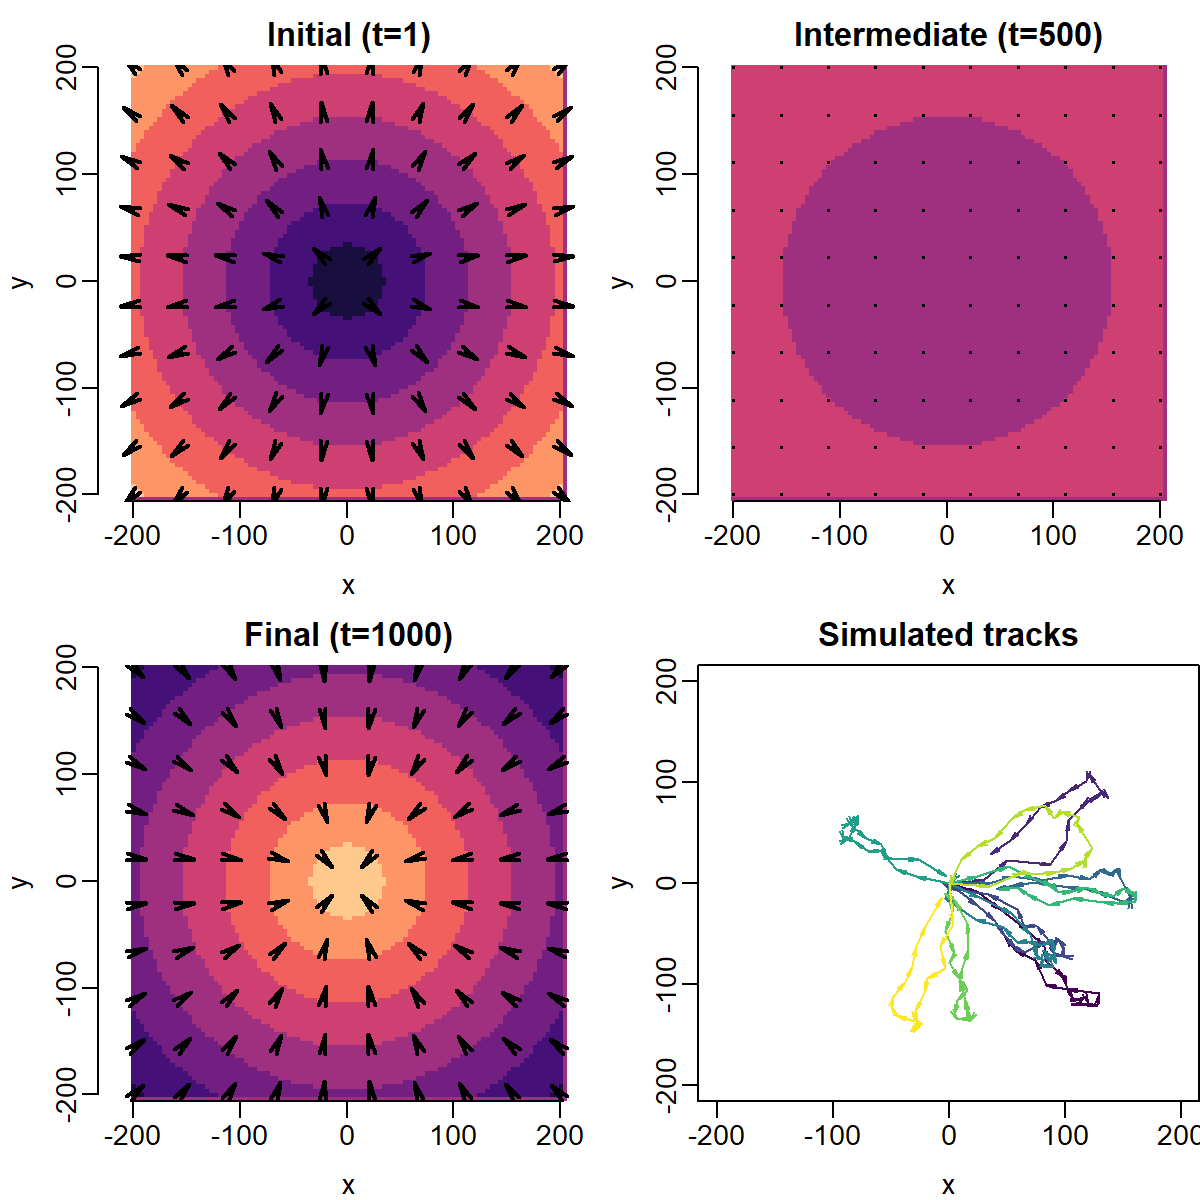
\includegraphics[width=5.5in]{Chap_4/Preference.png}
    \label{fig:Chap4_simulation}
\end{figure}

\section{Track Reconstruction} \label{sec:Chap4_track_reconstruction}

In Section \ref{sec:Chap4_diffusion_and_taxis}, we showed that we can simulate movement based on taxis (i.e., the gradient of a habitat preference function) and diffusion (otherwise unexplained changes in location).  However, applied ecologists often want to do this in reverse, i.e., infer movement processes and parameters from measurements of individual location, predict their location between measurements, and forecast future movement.  We next show how to fit this as a bivariate state-space model, while treating location \(\mathbf{s}\) as continuous valued and discretizing time \(t\) into intervals with duration \(\Delta_t\).  We first specify a model that attributes all movement to ``diffusion" (i.e., has no explanatory variables for passive drift or taxis).  In this model, we specify that animal location \(\mathbf{s}\) follows a multivariate random walk over time:

\begin{equation} \label{eq:Chap4_diffusive_movement}
    \mathbf{s}_{t+\Delta_t} \sim \mathrm{MVN}( \mathbf{s}_t, \Delta_t \mathbf{V})    
\end{equation}
where \(\mathbf{V} = \sigma_s^2 \mathbf{I}\) and \(\mathbf{I}\) is an identity matrix, such that \( \sigma_s^2 \Delta_t \mathbf{I} \) is the variance that accumulates over time \(\Delta_t\) at rate \(\sigma_s^2\).  Specifying the same diffusion rate in both spatial coordinates is sometimes called \myindex{isotropic}, and we will later extend the model to specify different or correlated diffusion rates in different directions by replacing \(\mathbf{I}\) with a different symmetric matrix.  

We complete the model by specifying a distribution for measurement errors:

\begin{equation} \label{eq:Chap4_measurement_distribution}
    \mathbf{y}_t \sim \mathrm{MVN}( \mathbf{s}_t, \sigma_y^2 \mathbf{I})    
\end{equation}
where we here assume that measurement error variance \( \sigma_y^2\) is known (i.e., from the error of a Global Positioning System measurement calculated based on the number and position of GPS satellites during the measurement). This model is similar to the previous state-space Gompertz population model (Eq. \ref{sec:Chap3_state_space}), although it now involves a multivariate normal distribution for both process and measurement errors.

This model can be specified in TMB using a few new concepts and model components (Code \ref{code:chap4-crawlTMB}).  We estimate animal location \colorbox{backblue}{x\_iz} at \colorbox{backblue}{i} times separated by intervals \colorbox{backblue}{DeltaT\_i}, fitted to data \colorbox{backblue}{y\_iz}.  Similar to Code \ref{code:Chap3-TMB-state-space}, we use function \colorbox{backblue}{R\_IsNA} to allow the model to detect and skip data that are missing, while still predicting animal location during those times.  Later, we will use this option to extract predictions of location between measurements (and associated standard errors), and it could also be used to forecast movement after the last available measurement. We use a function \colorbox{backblue}{density::MVNORM} that is included in a TMB library \colorbox{backblue}{density} to calculate a multivariate normal density from a specified covariance function. This \myindex{density library} will come in handy throughout the subsequent chapters as a compact way of specifying spatial and temporal correlations. We have also defined a function \colorbox{backblue}{make\_covariance} which assembles the covariance matrix for diffusion.  So far, we are defining \( \mathbf{V}=\sigma_s^2 \Delta_t \mathbf{I} \) but we include this function to allow other, more complicated versions for the covariance matrix which we introduce in later sections. Finally, we also include covariates \colorbox{backblue}{X\_ij} and covariate-response parameters \colorbox{backblue}{beta\_jz}, which we also introduce later, and define a matrix \colorbox{backblue}{Gsum\_iz} that calculates a cumulative sum of movement resulting from covariates.     

\lstset{style=TMBcode}
\lstinputlisting[language=c++, label=code:chap4-crawlTMB, caption=TMB code for specifying a bivariate state-space model for animal movement from a Lagrangian perspective., captionpos=t]{Chap_4/crawlTMB.cpp}

Before running the model, we check the sparsity of the inner Hessian matrix and confirm that every row of the Hessian is nonzero for at most three columns (Fig. \ref{fig:Chap4_hessian}).  Intuitively, this makes sense, given that the location \( x_{t} \) for spatial coordinate \(x\) depends upon the values of \( ( x_{t-1}, x_{t+1}, y_{t} ) \), and is independent of all other values conditional upon these three. 

\begin{figure}[!ht]
    \caption[Sparsity pattern for 2D autoregressive state-space model]{Illustration of the sparsity of the inner Hessian matrix for the two-dimensional track-reconstruction using a first-order autoregressive process for diffusion.}
    \centering
    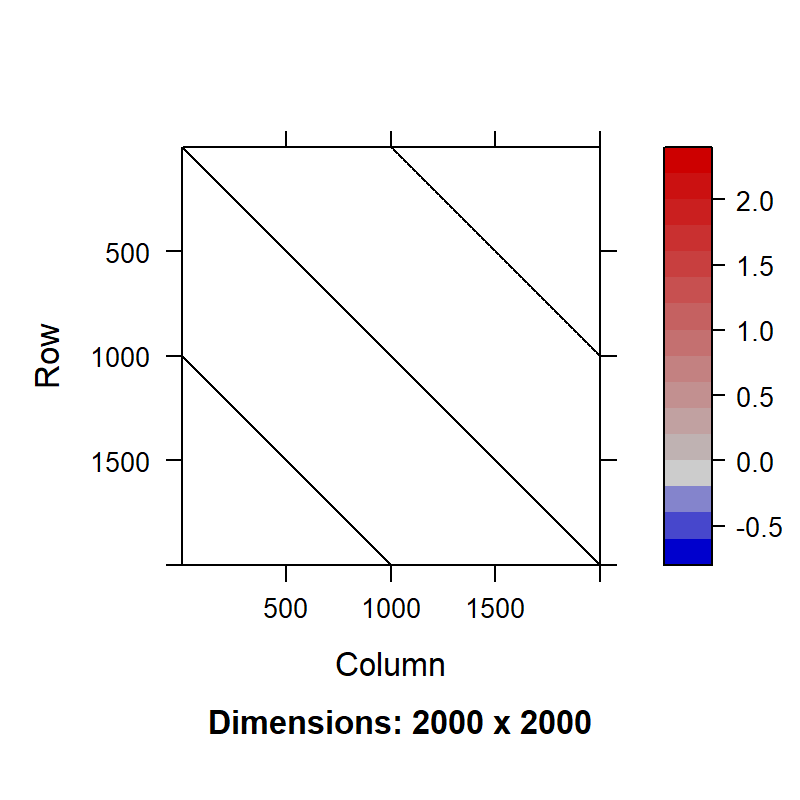
\includegraphics[width=4in]{Chap_4/sparsity.png}
    \label{fig:Chap4_hessian}
\end{figure}

We then fit this model in R only using data for 50 of the 1000 simulated time-steps (Code \ref{code:Chap4-R-fitted-individual}), which we accomplish by including \colorbox{backcolour}{NA} values for 950 measurements.  This model then allows us to predict location for all 1000 modeled times (Fig. \ref{fig:Chap4_fitted_diffusion}).  Given that we are fitting only 50 observations, the empirical Bayes prediction for movement follows 49 straight line-segments that connect each observation to the one before and after it (green lines). However, the model also estimates that uncertainty (i.e., the standard error on the random effect representing location) is lowest at the time of observations, and uncertainty increases and then decreases between any two observations.  This is sometimes called a \myindex{Brownian bridge}, where a Brownian (random-walk) process is used to predict an increase and subsequent decrease in predictive variance between two observations.

\lstset{style=Rcode}
\lstinputlisting[language=R, label=code:Chap4-R-fitted-individual, firstline=80, lastline=103, caption=R code fitting diffusive movement to location measured for a single individual., captionpos=t]{Chap_4/Simulate_movement.R}

\begin{figure}[!ht]
    \caption[Reconstructed track using bivariate autoregressive state-space model]{Illustration of a single simulation for the true location in each time (black dots), reconstructed tracks (green arrows), and uncertainty ellipse for each time (blue opaque circles).}
    \centering
    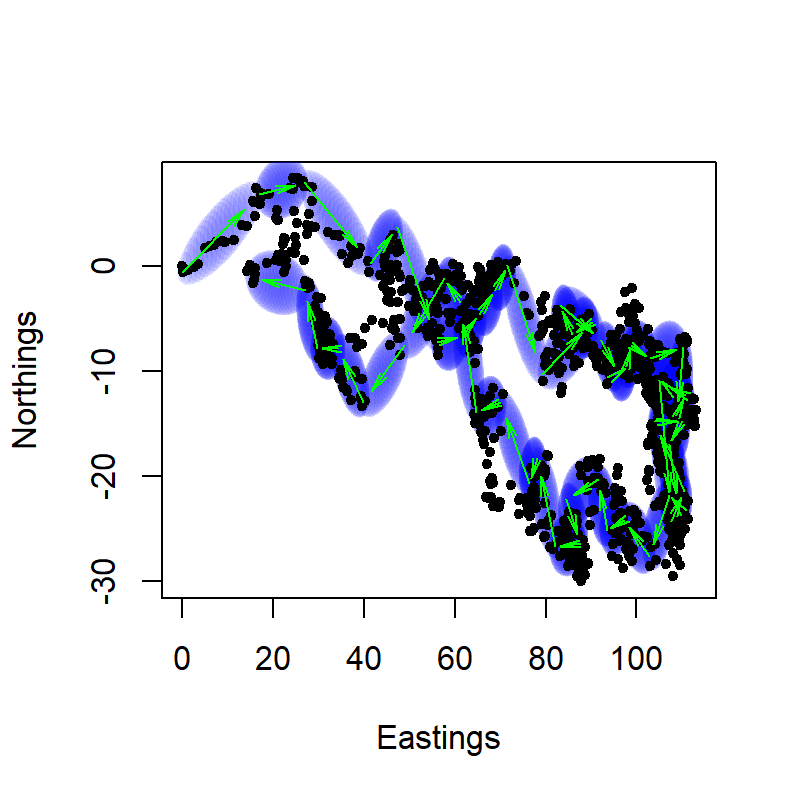
\includegraphics[width=4in]{Chap_4/fitted_diffusion.png}
    \label{fig:Chap4_fitted_diffusion}
\end{figure}

Next, we expand the model by approximating taxis (i.e., advection toward a preferred habitat) using a drift term (i.e., advection in a general direction without specifying a habitat preference function).  To do so, we expand Eq. \ref{eq:Chap4_diffusive_movement} to include a draft term in the mean of the multivariate normal distribution:

\begin{equation}
    \mathbf{s}_{t+\Delta_t} \sim \mathrm{MVN}( \mathbf{s}_t + \mathbf{z}_t \mathbf{B}, \Delta_t \mathbf{V})    
\end{equation}
where \( \mathbf{Z} \) is a matrix of covariates \( \mathbf{z}_t \) applied to each time-interval \(t\), and \( \mathbf{B} \) is a matrix of coefficients that measure the response for each covariate (rows) for each locational coordinate (columns), such that \(\mathbf{z}_t \mathbf{B}\) is the direction and magnitude of drift at time \(t\).  In the following, we specify a drift term as a cubic spline (using \colorbox{backcolour}{splines::bs} to construct the spline) for the time since the foraging trip began (Code \ref{code:Chap4-spline-for-drift}).  This drift term then approximates the tendency for an animal to follow a general heading over a prolonged period.  For a central-place forager, in particular, we assume that the drift term will tend to sum to zero over time, such that the animal has a tendency to ``drift" back to it's initial location. To explore this, we have already defined \colorbox{backblue}{Gsum\_iz} as a matrix that calculates the cumulative sum of  advection that is predicted by the drift term \( \mathbf{z}_t \mathbf{B} \), and we envision that \colorbox{backblue}{Gsum\_iz} will tend to end at a location that is near the start location.  We then compare this fit including diffusion and drift (Fig. \ref{fig:Chap4_fitted_drift}), with the previous fit that only included diffusion (Fig. \ref{fig:Chap4_fitted_diffusion}).  This comparison shows that including the drift term in this single track results in a small reduction in the uncertainty ellipse (a smaller blue-shaded area), but otherwise has little impact on the overall estimate of the animal track. 

\lstset{style=Rcode}
\lstinputlisting[language=R, label=code:Chap4-spline-for-drift, firstline=130, lastline=138, caption=R code to generate basis functions representing a cubic spline for the drift term and then rebuilding the TMB model., captionpos=t]{Chap_4/Simulate_movement.R}
 

\begin{figure}[!ht]
    \caption[Reconstructed track with estimated drift using bivariate model]{Same as \ref{fig:Chap4_fitted_diffusion}, but also showing the cumulative sum of the drift term (red line), calculated by setting diffusion to zero in the fitted object. We include this to visualize the aggregate effect of the drift term on predicted location, where the start and end location of the red line are close to one another, as expected for a central-place forager.}
    \centering
    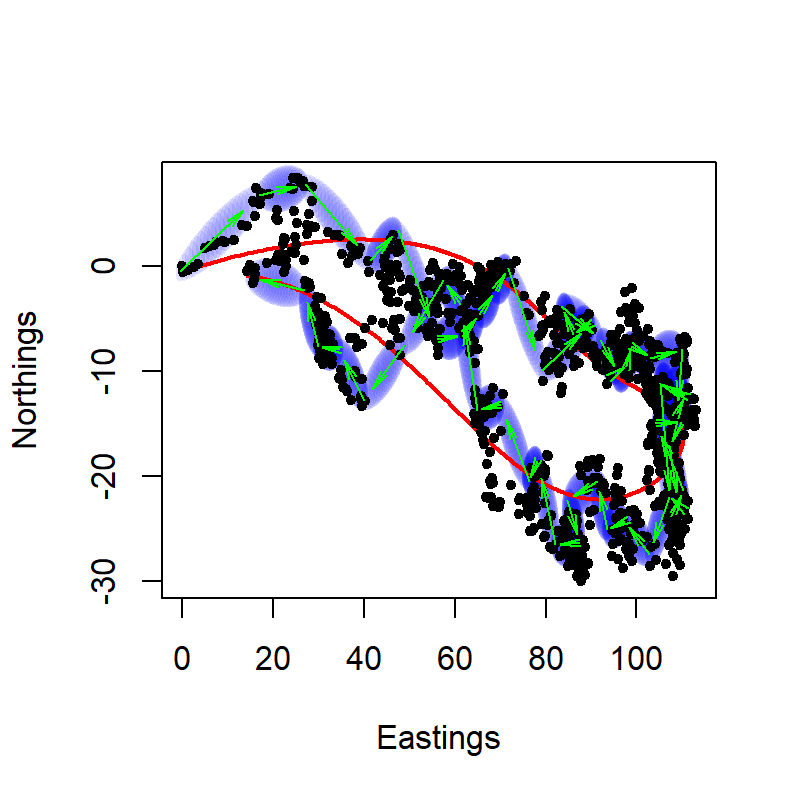
\includegraphics[width=4in]{Chap_4/fitted_drift.png}
    \label{fig:Chap4_fitted_drift}
\end{figure}

Similarly, we can fit this same model to locational data for a northern fur seal (\textit{Callorhinus ursinus}), specifically a lactating adult female, that was tagged at St. Paul Island in 2016 (Fig. \ref{fig:Chap4_NFS}).  The data are obtained using a GPS tag and have been analyzed elsewhere \cite{kuhn_test_2020}.  We thin the 237 GPS location records to 25 measurements, and compare the predicted track with the withheld measurements.  This analysis shows again that a basis spline for the time since the trip started can predict some but not all of the movement, and that the standard errors generally are similar to the withheld measurements.  

\begin{figure}[!ht]
    \caption[Reconstructed track and drift using northern fur seal data]{Same as \ref{fig:Chap4_fitted_drift}, but fitted to data for a northern fur seal foraging trip from St. Paul Island in 2016 where x and y coordinates in the Universal Transverse Mercator (UTM) zone-2 projection.}
    \centering
    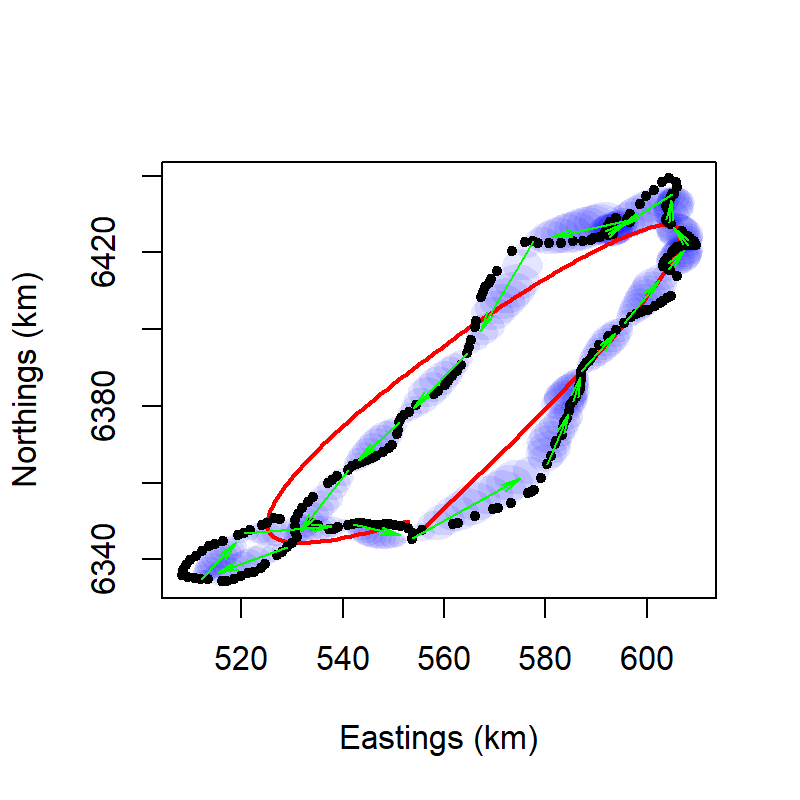
\includegraphics[width=4in]{Chap_4/fitted_NFS.png}
    \label{fig:Chap4_NFS}
\end{figure}

\section{Specifying Covariance Matrices} \label{eq:Chap4_covariance_matrices}

So far, we have explored a bivariate state-space model, which includes a state vector \( \mathbf{s}_t = (x_t,y_t) \) which describes the location of a single animal using two spatial coordinates.  However, many state-space models will involve more than two variables.  For example, we might seek to describe:
\begin{itemize}
    \item Abundance for multiple species in a community using a vector autoregressive model.  For example, we might define \( \log( \mathbf{n}_{t+1}) = \mathbf{\alpha + B} \log(\mathbf{n}_{t})\) where \(\mathbf{B}\) is a matrix of community interactions and \(n_{c,t}\) is abundance for each species \(c\).  This results in a multivariate version of the Gompertz model for population dynamics \cite{ives_estimating_2003,thorson_estimating_2017}.  In this case, many properties of community dynamics can be calculated from the matrix \(\mathbf{B}\) of species interactions; 

    \item Size-at-age for multiple ages \cite{stawitz_state-space_2015}, used to identify environmental drivers that might affect individual growth rates;

    \item Juvenile survival rates for different habitats in a spatially structured meta-population \cite{minto_productivity_2014}, used to identify demographic stability for the entire species.
\end{itemize}  
In these and other cases, we might want to estimate the correlation between different variables, and therefore need to replace the diagonal covariance \( \mathbf{V} = \sigma_s^2 \mathbf{I} \) with a general covariance matrix.  However, as the number of variables \(N\) increases, the number of correlation and variance parameters in an unstructured covariance matrix is \(N(N+1)/2\), and this becomes prohibitive as \( N>>10 \).  

We first summarize four alternative parameterizations of the covariance matrix \( \mathbf{V} \) before discussing them in detail subsequently: 
\begin{enumerate}
    \item \textit{Diagonal and equal}:  this is what we've been using so far, \( \mathbf{D}_{equal} = \sigma^2 \mathbf{I} \), and it involves a single parameter, which is easiest to specify as \( \sigma^2 = \mathrm{exp}(\theta) \);

    \item \textit{Diagonal and unequal}:  aternatively, we might specify that each variable has a unique variance. For example, if modelling three variables this will result in:
    
\begin{equation}
    \mathbf{D}_{unequal} = \begin{bmatrix}
    \sigma_1^2 & 0 & 0 \\
    0 & \sigma_2^2 & 0 \\
    0 & 0 & \sigma_3^3
    \end{bmatrix}    
\end{equation}
    This parameterization involves \(N\) parameters but still specifies that variables are independent;

    \item \textit{Factor model}:  we might instead specify a factor model and use this to generate the covariance matrix.  This factor model can range in complexity.  For example, it could represent a single exogenous driver that explains variation in all variables.  Alternatively, it can be used to represent an unstructured covariance matrix;  

    \item \textit{Structural equation model}:  finally, we might specify a structural equation model and use this to calculate the resulting covariance among factors.  This approach allows correlations to be derived from parameters that are interpreted as regression slopes.  However, it also requires specifying the structural relationship among variables a priori. 
\end{enumerate}
We next discuss computational details regarding Factor and Structural Equation Modelling approaches to covariance.   
 
\subsection{Factor Models} \label{sec:Chap4_factor_model} 
We might envision that the covariance among variables arises from a \myindex{factor model} with \(N_{factors}\) axes of covariation.  
    
\begin{equation} \label{eq:Chap4_factor_model}
    \mathbf{V}_{factor} = \mathbf{\Lambda} \mathbf{\Lambda}^T    
\end{equation}
where \(\mathbf{\Lambda}\) is a matrix with \(N\) rows and \(N_{factors}\) columns.  Eq. \ref{eq:Chap4_factor_model} is only identifiable given further restrictions on parameters \cite{zuur_dynamic_2003,zuur_estimating_2003}.  We choose to ensure identifiability by specifying that any element above the diagonal is fixed at zero.  For example, when \(N=3\) and \(N_{factors}=2\) we get:
\begin{equation} \label{eq:Chap4_loadings_matrix}
    \mathbf{\Lambda} = \begin{bmatrix}
    \lambda_{1,1} & 0  \\
    \lambda_{2,1} & \lambda_{2,2} \\
    \lambda_{3,1} & \lambda_{3,2}     
    \end{bmatrix}    
\end{equation}
This factor model can be interpreted in several ways:

\begin{enumerate}
    \item \textit{Trimmed Cholesky matrix}: as one interpretation, recall that covariance \(\mathbf{V}\) is a symmetric matrix, and we can calculate a \myindex{Cholesky decomposition} of any symmetric matrix where \(\mathbf{V = LL}^T\) and \(\mathbf{L}\) is a lower-triangle matrix (i.e., has value 0 above the diagonal, see Section \ref{sec:Appendix_Cholesky} for details).  In Eq. \ref{eq:Chap4_loadings_matrix}, we are therefore estimating \(N_{factor}\) columns of the Cholesky matrix, and we therefore call it a \textit{trimmed Cholesky} matrix.  When \(N=N_{factors}\), the loadings matrix \(\mathbf{\Lambda}\) is the full Cholesky matrix, \colorbox{backcolour}{L = chol(V)}, and \(\mathrm{V}_{factor}\) is full rank.  Estimating all parameters in this Cholesky matrix is then equivalent to estimating an \textit{unstructured covariance}, and it involves estimating as many parameters as are identifiable. Alternatively, when \(N_{factors}<N\), the resulting \(V_{factor}\) has rank \(N_{factors}<N\) and it involves estimating fewer parameters;   

    \item \textit{Loadings matrix}: we use the symbol \(\mathbf{\Lambda}\) (the Greek letter for L) to indicate that it can be interpreted as a \myindex{loadings matrix} where, e.g., \(\lambda_{2,1}\) represents how strongly variable 2 is loaded on (i.e., associated with) factor 1.     
\end{enumerate}

To illustrate these two interpretations of the factor-model covariance, consider that we have a vector \(\mathbf{x}\) composed of standard normal random variables:

\begin{equation}
    \mathbf{x} \sim \mathrm{MVN}( \mathbf{0}, \mathbf{I} )    
\end{equation}
If we then take the product of this and the loadings matrix:

\begin{equation}
    \mathbf{y} = \mathbf{\Lambda x}    
\end{equation}
the resulting vector \(\mathbf{y}\) can be written as:

\begin{equation}
    \mathbf{y} \sim \mathrm{MVN}( \mathbf{0}, \mathbf{V}_{factor} )    
\end{equation}
where \( \mathbf{V}_{factor} = \mathbf{\Lambda \Lambda}^T \). We can therefore interpret the loadings matrix \( \mathbf{\Lambda} \) either (1) as a projection matrix that transforms latent factors \(\mathbf{x}\) into the response variable \(\mathbf{y}\), or (2) as a tool to construct the covariance \( \mathbf{V}_{factor} \).  The former interpretation is useful, e.g., to decompose a multivariate process with \(N\) variables into a simpler process involving \(N_{factor}\) factors.  For example, this is commonly done during species ordination, where a vector of species densities at different sites is reduced to two axes, and the loadings \( \mathbf{\Lambda}^T \) and factors \( \mathbf{x} \) are plotted on a two-dimensional scatterplot \cite{mccune_analysis_2002}.  

In practices, there are two caveats to using the factor-model covariance.  
\begin{itemize}
    \item \textit{Ensuring full rank}:  when using a rank-reduced factor model, \(N_{factors}<N\), it may still be convenient to ensure that the covariance is full rank.  This ensures that any possible vector \(\mathbf{y}\) is within the support of the covariance (i.e., the null space is an empty set).  To achieve this, we often use:
\begin{equation}
    \mathbf{y} \sim \mathrm{MVN}( \mathbf{0}, \mathbf{\Lambda \Lambda}^T+\mathbf{D} )   
\end{equation}
    where \(\mathbf{D}\) is diagonal and either equal or unequal;

    \item \textit{Rotations}:  similarly, we have specified that the loadings matrix \(\mathbf{\Lambda}\) is lower-triangle;  this constraint ensures that columns cannot be freely rotated, and hence ensures identifiability.  However, factors cannot be interpreted independently of one-another.  Ecologists therefore typically ``rotate" factors prior to interpreting them:
\begin{equation} \label{eq:Chap4_rotations}
\begin{gathered}
    \mathbf{x}^* = \mathbf{Hx} \\
    \mathbf{\Lambda}^* = \mathbf{\Lambda H}^{-1} 
\end{gathered}    
\end{equation}
    where \( \mathbf{H} \) is the \myindex{rotation matrix}.  It is then easy to see that this rotation leaves the model unchanged, where \( \mathbf{y} = \mathbf{\Lambda x} = \mathbf{\Lambda}^*\mathbf{x}^* \) for any invertible matrix \(\mathbf{H}\).  Ecologists typically use a \myindex{varimax rotation}, which ensures that loadings \(\mathbf{\Lambda}^*\) has a few large values and many small values (i.e., factors typically represent a small number of individual variables).  However, we also use a \myindex{principal component analysis rotation} \cite{thorson_joint_2016}, where the first axis explains as much variance as possible, the 2nd explains as much as possible given this, etc.  This rotation then ensures that the first axis is the ``dominant mode of variability", and that displaying only the first two axes still captures as much of the total variance as possible.
\end{itemize}

\subsection{Structural Equation Models} \label{sec:Chap4_SEM}
Alternatively, an analyst may have a priori knowledge about associations between variables.  In the strongest case, the analyst might specify a \myindex{causal map}, e.g., specifying that changing variable \(X_1\) causes a change in variable \(X_2\), \(X_1\) and \(X_2\) both cause a change in \(X_3\), and \(X_3\) causes a change in \(X_4\), which in turn affects \(X_1\).  These types of cycles are common in trophic relationships where species are often assembled in tightly interacting \textit{trophic modules} with weak linkages between modules \cite{holt_community_1997}.  Additionally. this type of graphical model or causal map often arises from eliciting stakeholder input, where input can be used to generate a \textit{conceptual model} of ecosystem function, which then be represented as a \myindex{structural equation model} \cite{kaplan_structural_2001}:

\begin{equation}
    \mathbf{y} = \mathbf{\Rho y} + \mathbf{\delta}    
\end{equation}
where \( \mathbf{\Rho} \) is a matrix of path coefficients that represent the hypothesized linear relationships linking variables, and \( \mathbf{\delta} \sim \mathrm{MVN}(\mathbf{0},\mathbf{\Sigma}) \) represents additional exogenous drivers.  This then results in a covariance:

\begin{equation} \label{eq:Chap4_SEM_covariance}
    \mathrm{Var}(\mathbf{y}) = \mathbf{B} \mathbf{\Sigma} \mathbf{B}^T    
\end{equation}
where \( \mathbf{B} = (\mathbf{I-\Rho})^{-1} \) and \( \mathbf{\Sigma=\Lambda \Lambda}^t \). Structural equation packages in R \cite{fox_sem_2020} typically combine this calculation with an inverse-Wishart distribution for the sample covariance from a set of measurements, but the procedure for converting mechanisms \( \mathbf{\Rho} \) and \( \mathbf{\Gamma} \) to a covariance can then be used in any nonlinear model.  

Specifying covariance using a structural-equation model has several benefits \cite{thorson_identifying_2023}:
\begin{enumerate}
    \item \textit{Parsimonious representation}:  it allows detailed control over how many parameters \(N_{sem}\) are used to represent the relationship among variables.  In particular, SEM can estimate any number of parameters from \(N_{sem}=1\) (i.e., \(\mathbf{\Lambda} = \sigma \mathbf{I}\)) to \(N_{sem} = N(N+1)/2 \) to represent the covariance, where \(N\) is the number of variables;

    \item \textit{Complex and cyclic ecological relationships}:  the SEM can include cyclic dependencies (e.g., a trophic flow from resource to producer to consumer, but where the consumer increases the basal resource via excretion) as long as the total number of dependencies (\(N_{sem}\)) is less than the degrees of freedom in the covariance matrix, \(N_{sem} \leq N(N+1)/2 \); 

    \item \textit{Conceptual modelling}: the structural equations can often be generated from existing conceptual or semi-quantitative models for a given ecological system;

    \item \textit{Path coefficients as regression slopes}:  the estimated coefficients in \(\Rho\) are interpreted similarly to regression slopes in a linear model, i.e., a change of \(\Delta\) in \(y_1\) causes a \(\rho_{2,1} \Delta\) change in \(y_2\).
\end{enumerate}
However, the resulting estimates depend upon the structural equation model that is specified, so model-building requires additional information about the system that is explicitly represented by the SEM. 

\section{Comparing Factor and Structural Equation Models for Group Movement} \label{Section:Chap4_comparing_factor_and_SEM}

We therefore have a wide range of methods available for specifying a covariance matrix among variables.  These different options are implemented in the TMB custom function \colorbox{backblue}{make\_covariance} (Code \ref{code:Chap4-custom-function}).  We next demonstrate this using simulated data, representing 10 tracked individuals that pursue a similar foraging strategy that involves moving northward and then returning toward their starting location (Code \ref{code:Chap4-R-movement-fitting}).  This shared foraging strategy results in correlated random walks that are correlated along the y-axis but not the x-axis across individuals (see Fig. \ref{fig:Chap4_Preference_correlated}).

\lstset{style=TMBcode}
\lstinputlisting[language=c++, label=code:Chap4-custom-function, caption=Custom function \colorbox{backblue}{make\_covariance} used to construct a covariance among species using a factor model or structural equation model., captionpos=t]{Chap_4/make_covariance.hpp} 

\lstset{style=Rcode}
\lstinputlisting[language=R, label=code:Chap4-R-movement-fitting, firstline=187, lastline=222, caption=R code fitting a multivariate state-space movement model to location measurements for multiple animals from a Lagrangian perspective., captionpos=t]{Chap_4/Simulate_movement.R}

\begin{figure}[!ht]
    \caption[Simulated movement for correlated tracks of central-place foragers]{Same as \ref{fig:Chap4_simulation}, but modified such that individuals tend to leave heading northward before returning toward their original location.}
    \centering
    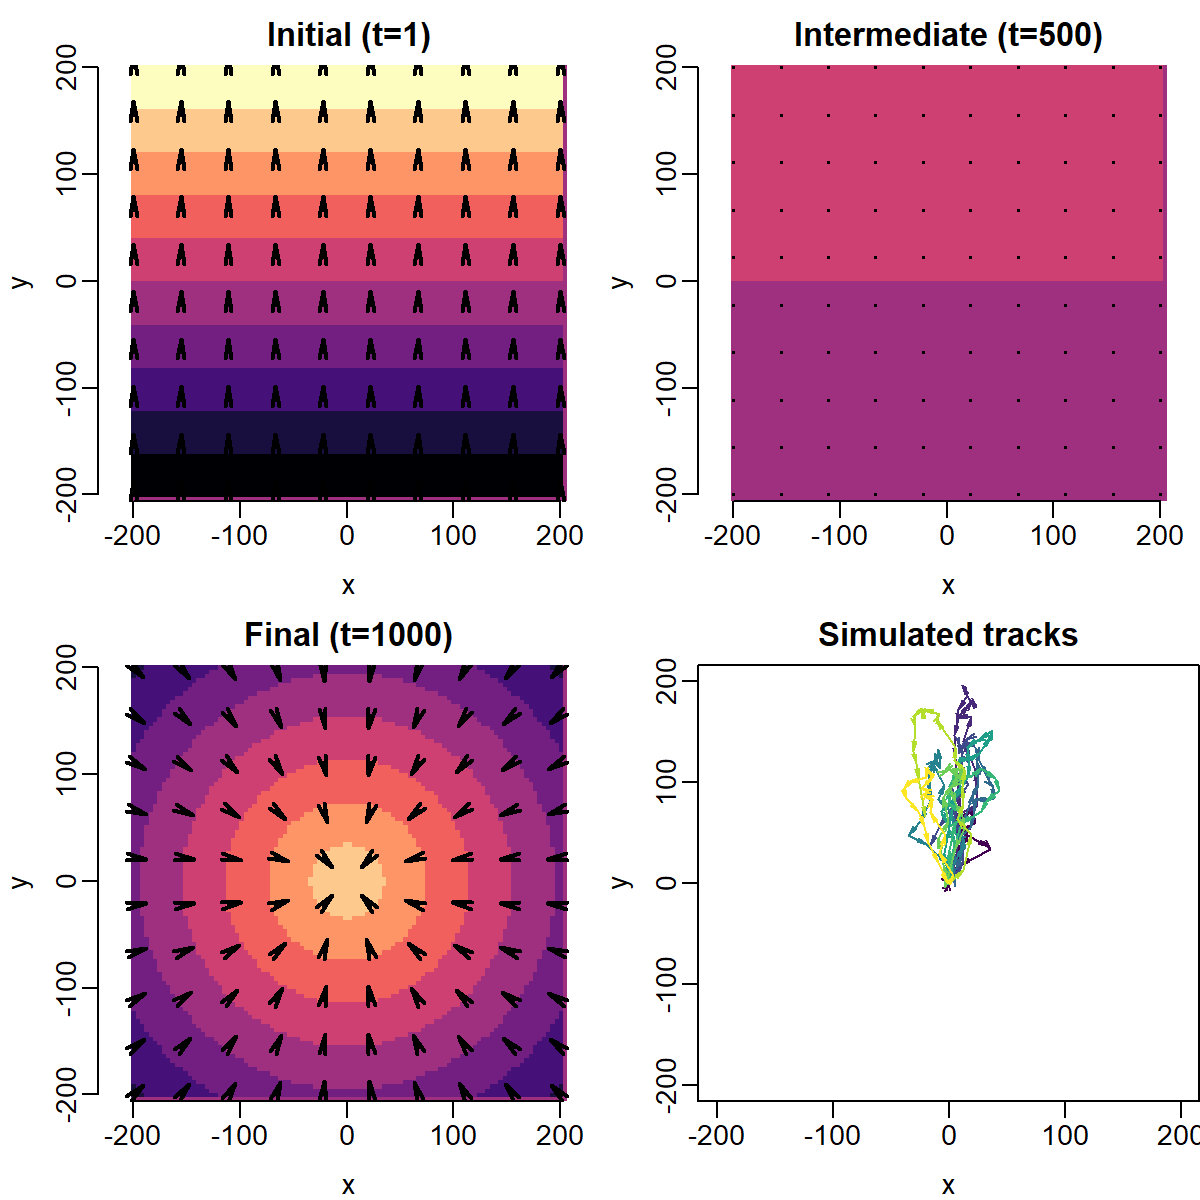
\includegraphics[width=4in]{Chap_4/Tracks-Correlated.png}
    \label{fig:Chap4_Preference_correlated}
\end{figure}

We then fit this model again using the three alternative approaches to specifying the covariance in diffusion among animals (i.e., specifying \( \mathbf{V} \) in Eq. \ref{eq:Chap4_diffusive_movement}):
\begin{enumerate}
    \item The ``diagonal-and-equal" covariance matrix \( \mathbf{V} = \mathbf{D}_{equal} \) where \(\mathbf{D}_{equal} = \sigma^2 \mathbf{I} \), involving one parameter representing covariance among individuals;

    \item An alternative factor-model covariance, \( \mathbf{V} = \mathbf{D}_{equal} + \mathbf{\Lambda \Lambda}^T \) using \( N_{factors}=2 \) under the assumption that there's potential correlations in x- and y-axis directions.  This then results in 16 parameters representing covariance (15 in the factor model, and one more in the diagonal-and-equal matrix);

    \item A structural equation-model covariance, under the assumption that animal \#1 is leading the other animals and therefore movement for that animal then causes similar movement for the others.  This specification results in 2 estimated parameters representing the impact of animal \#1 on other animals, for each of two spatial coordinates.  
\end{enumerate}
We specify the structural equation model by writing a text file that is parsed by function \colorbox{backcolour}{specifyModel} in R-package \colorbox{backcolour}{sem} \cite{fox_sem_2020} (Code \ref{code:Chap4-build-ram}).  This text file is used to specify which path coefficients should be estimated in \( \mathbf{\Rho} \) and these are indicated by using a single-headed arrow where, e.g., \colorbox{backcolour}{y1 -$>$ y2} indicates that the model should estimate the magnitude of change in \colorbox{backcolour}{y2} expected from a change in \colorbox{backcolour}{y1}.  This text file is also used to specify which parameters should be estimated in the Cholesky \( \mathbf{\Lambda} \) of exogenous variance \(\mathbf{\Sigma}\).  These are indicated by using a double-headed arrow where, e.g., \colorbox{backcolour}{y1 $<$-$>$ y1} indicates that the variance of \colorbox{backcolour}{y1} should be estimated, or \colorbox{backcolour}{y1 $<$-$>$ y2} indicates that the covariance of \colorbox{backcolour}{y1} and \colorbox{backcolour}{y2} should be estimated.  By specifying \colorbox{backcolour}{exog.variances=TRUE}, \colorbox{backcolour}{specifyModel} automatically adds a two-headed arrow for each variable, i.e., estimates a diagonal and unequal matrix for exogenous covariance \(\mathbf{\Epsilon}\).  Finally, the text file requires the user to specify a label for each parameter (i.e., in each row).  When two or more parameters share a single label (e.g., all path coefficients are named \colorbox{backcolour}{y} in this example), then those coefficients are all estimated to have the same value.  Similarly, if a parameter is labeled \colorbox{backcolour}{NA}, then they are fixed at a value \textit{a priori} that is provided immediately after the parameter name.  This text file is then parsed by a custom function \colorbox{backcolour}{build\_ram} that constructs a matrix \colorbox{backcolour}{RAM}, which is used in turn by \colorbox{backblue}{make\_covariance} to construct the covariance given model parameters (see Code \ref{code:Chap4-custom-function}). 

\lstset{style=Rcode}
\lstinputlisting[language=R, label=code:Chap4-build-ram, firstline=264, lastline=274, caption=R interface to build a Structural Equation Model for group movement., captionpos=t]{Chap_4/Simulate_movement.R}

These three hypotheses therefore provide a wide range of model complexity, and illustrate different avenues to specify a covariance matrix.  Similarly, they result in a range of different estimates of covariance among variables (Fig. \ref{fig:Chap4_joint_covariance}), although the factor and structural-equation estimates of covariance both correctly identify a large covariance among individuals in movement along the y-axis.  The Akaike Information Criterion identifies that the factor-model covariance is most parsimonious, despite having the most parameters (see bottom-right of each panel in Fig. \ref{fig:Chap4_joint_tracks}).  Despite these differences, however, all models estimate tracks that are almost indistinguishable (Fig. \ref{fig:Chap4_joint_tracks}).  This then suggests that the data are sufficiently informative that these small differences in model structure have little leverage over interpolated locations.  

\begin{figure}[!ht]
    \caption[Estimated covariance in movement using alternative correlation methods]{Covariance in movement \(\mathbf{V}\) in Eq. \ref{eq:Chap4_diffusive_movement} visualized using the function \colorbox{backcolour}{corrplot} in the \colorbox{backcolour}{corrplot} package \cite{wei_r_2021}, where the area of each circle is proportional to the covariance (and see the colorbar legend at the bottom of each panel), for the diagonal-and-unequal covariance (left panel), factor model (middle panel), or structural equation model (right panel), and the 8 variables are labeled x or y for movement in eastings or northings, respectively, and are also labeled 1 through 4 for the four animals.}
    \centering
    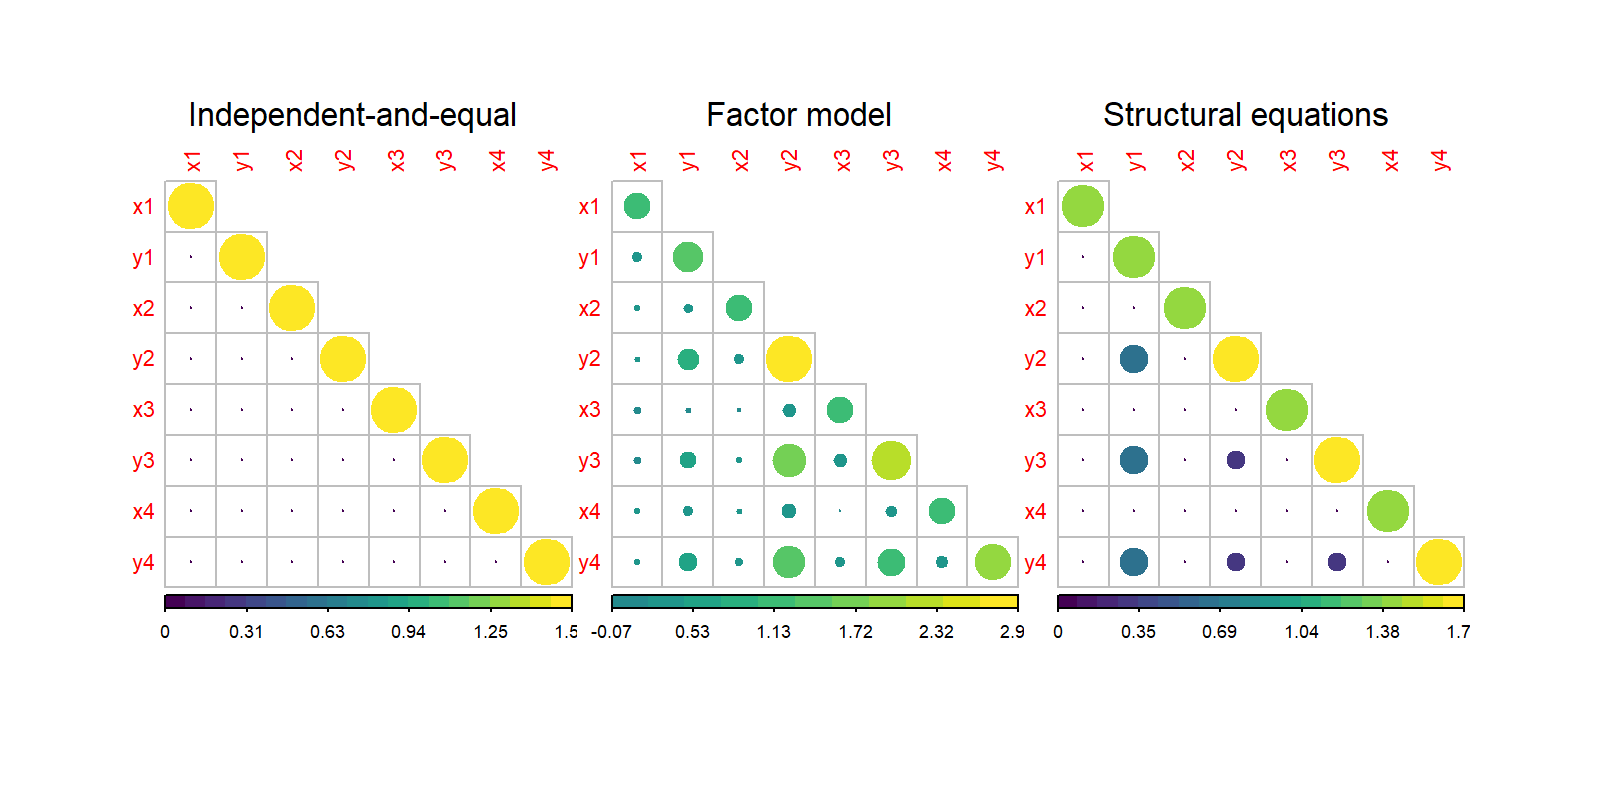
\includegraphics[width=5.5in]{Chap_4/fitted_joint-covariance.png}
    \label{fig:Chap4_joint_covariance}
\end{figure}

\begin{figure}[!ht]
    \caption[Reconstructed tracks using alternative correlation methods]{Depiction of reconstructed tracks for the 1st animal, following same plotting format as Fig. \ref{fig:Chap4_fitted_diffusion}, using the diagonal-and-unequal covariance (left panel), factor model (middle panel), or structural equation model (right panel).  We also list the Akaike Information Criterion (AIC) value for each model in the bottom-right of each panel, where the lowest value corresponds to the highest expected performance for new data (see Section \ref{sec:Chap1_evaluating_model_fit}).  In this case, the lowest AIC occurs using the factor-model covariance.  Differences in reconstructed track using these three covariance matrix structures were similarly small for the other three animals (results not shown here).}
    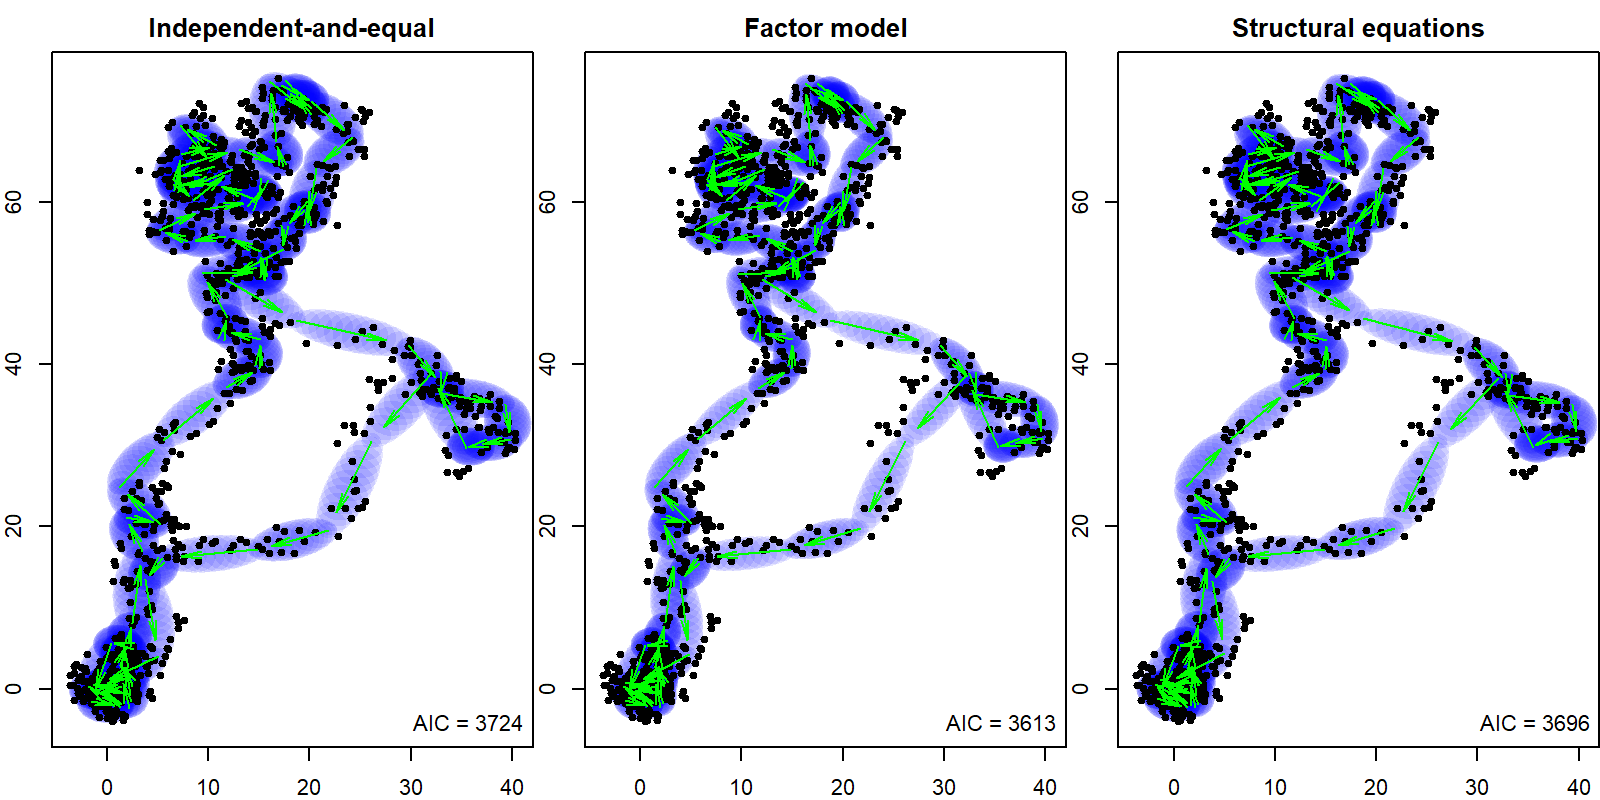
\includegraphics[width=5.5in]{Chap_4/fitted_joint-tracks.png}
    \label{fig:Chap4_joint_tracks}
\end{figure}

\section{Chapter Summary}

In summary, we have showed that:
\begin{enumerate}
    \item Individual movement can be described explicitly (by tracking individual position over time) or implicitly (by deriving properties arising from aggregating movement across time or individuals). It is possible to calculate ecological patterns arising from explicit consideration of organism movement, but harder to go in the reverse direction and derive organism movement processes from observed ecological patterns;

    \item Individual movement can be decomposed into three components representing taxis (movement toward preferred habitat), drift (movement in a specified direction), and diffusion (otherwise unexplained movement).  Taxis and drift are sometimes combined using the term advection.  These processes can be described in continuous space and time using a stochastic differential equation, or discretized in continuous space and discrete time as a difference equation;  

    \item Individual tracks arise from a movement in two dimensions, and can be simulated using taxis, drift, and diffusion.  Similarly, these tracks can be reconstructed using intermittent location measurements using a multivariate state-space model. In these cases, taxis can be approximated using a drift term if the covariates driving habitat preferences are unknown or unavailable;
    
    \item Tracks for multiple individuals can be reconstructed jointly using a multivariate state-space model with a larger number of position variables.  Large multivariate models involve a covariance matrix. If correlations are ignored, this can be approximated as ``diagonal-and-equal" or ``diagonal-and-unequal" matrices.
    
    \item Covariance among multiple time-series (representing animal locations or otherwise) can be estimated using a factor-model covariance. This factor model involves estimating a few columns of the Cholesky decomposition of covariance.  This can be interpreted as a loadings matrix, which measures the association of each variable with each latent factor. The factor model requires additional restrictions to ensure that results are identifiable, and results can be interpreted after applying a varimax or PCA rotation.  
    
    \item Alternatively, covariance among multiple time-series can be estimated using a structural-equation covariance matrix.  This approach yields path coefficients that are interpreted like standard regression slopes.  The structural-equation covariance allows detailed control over the number of estimated parameters, and can represent ecological assumptions about the causal mechanisms that operate among variables.  
\end{enumerate}

\section{Exercise}

In Section \ref{sec:Chap4_diffusion_and_taxis} and Code \ref{code:R-simulate-track}, we simulate tracks for a central-place forager such that preference initially increases with distance from the starting point but then reverses, such that the individual tends to move away and then back to the centroid of its range.  First, please modify this simulation to match an alternative ecological scenario of your choice, e.g., simulating daily movement where the animal has a normally distributed preference in summer and winter, but where the centroid differs between these seasons, such that they move from one to other range seasonally.  Then, calculate the expected habitat utilization given this preference function, e.g., by calculating 1000s of animal tracks, discretizing the spatial domain, and then calculating the proportion of time spent in each grid cell.  Consider changing the relative magnitude of diffusion vs. taxis (where the latter is controlled by the height of the preference function), and seeing how this affects the resulting habitat utilization.  

% \end{minipage}
% \end{center}